\documentclass[12pt,a4paper]{scrartcl}
\usepackage[utf8]{inputenc}
%\usepackage[latin1]{inputenc} %  Alternativ unter Windows
\usepackage[T1]{fontenc}
\usepackage[paper=a4paper,
left=25mm,
right=25mm,
top=25mm,
bottom=20mm]{geometry}
\usepackage[nottoc]{tocbibind}
\usepackage[ngerman]{babel}
\usepackage[pdftex]{graphicx}
\usepackage{latexsym}
\usepackage{amsmath}
\usepackage{amssymb,amsthm,amsfonts}
\usepackage{mathtools}
\usepackage{enumitem}
\usepackage[utf8]{inputenc}
\usepackage{float}
\usepackage{physics}
\usepackage{subfigure}
\usepackage{wasysym}
\usepackage{amssymb}
\newcommand{\R}{\mathbb{R}}


\DeclareMathOperator{\dive}{div}
\newtheorem{Satz}{Satz}[section]\newtheorem{Definition}[Satz]{Definition} 
\newtheorem{Lemma}{Lemma}		                 
\newtheorem{Korollar}[Satz]{Korollar}
\newtheorem{Proposition}[Satz]{Proposition}                  
\newtheorem{examples}[Satz]{Beispiel}
\let\oldexamples\examples
\renewcommand{\examples}{\oldexamples\normalfont}
\newtheorem*{notation}{Notation}
\let\oldnotation\notation
\renewcommand{\notation}{\oldnotation\normalfont}
\newtheorem*{remark}{Bemerkung}
\let\oldremark\remark
\renewcommand{\remark}{\oldremark\normalfont}                  
\newtheorem*{define}{Definition}
\let\olddefine\define
\renewcommand{\define}{\olddefine\normalfont}
\newtheorem*{repetition}{Wiederholung}
\let\oldrepetition\repetition
\renewcommand{\repetition}{\oldrepetition\normalfont}



\usepackage{bbm}
\usepackage[german=quotes]{csquotes}
\usepackage{xcolor}
\newcommand*\diff{\mathop{}\!\mathrm{d}}
\DeclareMathOperator{\conv}{conv}
\DeclareMathOperator{\spann}{span}
\DeclareMathOperator{\Jacobi}{D}
\DeclareMathOperator{\diam}{diam}
\definecolor{Mygreen}{RGB}{0,128,0}
\newcommand{\defi}[1]{\textcolor{Mygreen}{#1}}
%\renewcommand{\phi}{\varphi}
\renewcommand{\epsilon}{\varepsilon}
\newcommand{\unklar}[1]{\textcolor{blue}{#1}}
\newcommand\restr[2]{{% we make the whole thing an ordinary symbol
		\left.\kern-\nulldelimiterspace % automatically resize the bar with \right
		#1 % the function
		\vphantom{\big|} % pretend it's a little taller at normal size
		\right|_{#2} % this is the delimiter
}}
\newcommand{\cupdot}{\mathbin{\mathaccent\cdot\cup}}
\DeclareMathOperator{\sign}{sign}
\newcommand{\rhoin}{\rho_{\text{in}}}
\newcommand{\Gammain}{\Gamma_{{\text{in}}}}
\newcommand{\Gammaout}{\Gamma_{{\text{out}}}}
\newcommand{\GammaD}{\Gamma_{\text{D}}}
\newcommand{\GammaN}{\Gamma_{\text{N}}}
\newcommand{\GammaR}{\Gamma_{\text{R}}}
\DeclareMathOperator{\lTG}{(TG)}
\DeclareMathOperator{\swlTG}{(swTG)}
\DeclareMathOperator{\stlTG}{(stTG)}
\DeclareMathOperator{\Abb}{Abb}
\DeclareMathOperator{\supp}{supp}
\DeclareMathOperator{\sym}{sym}
\DeclareMathOperator{\KDR}{(KDR)}
\DeclareMathOperator{\sdKDR}{(sdKDR)}
\DeclareMathOperator{\vdKDR}{(vdKDR)}
\DeclareMathOperator{\OpKDR}{(Op-KDR)}
\DeclareMathOperator{\sDKDR}{(small-KDR)}
\DeclareMathOperator{\Pe}{Pe}
\DeclareMathOperator{\CinV}{C_{\text{inV}}}
\DeclareMathOperator{\SD}{\text{SD}}

\numberwithin{equation}{section} 


% Praktikumsbericht nummer setzen
\newcommand{\BerichtNR}{4}

\begin{document}
\begin{titlepage}
	
\includegraphics[scale=0.5]{kit-logo.jpg} 
	\begin{center} 
		\LARGE 
		\vspace*{2cm}
		\LARGE Praktikumsbericht \BerichtNR
		\vspace*{1.0cm}
		\hrule
		\vspace*{0.2cm}
		{\vspace{0.2cm} \huge Einführung in das Wissenschaftliche Rechnen}\vspace{0.5cm}
		\hrule
		\vspace*{2.5cm}
		\Large Stefan Karch \\
		Florian Döttling \\
		Tim Buchholz  \\
		\vspace*{1cm}
		20.05.2019 \\
		\vspace*{1.5cm}
		\vspace*{4.0cm}
		\Large Betreuung: Prof. Dr. Christian Wieners, Niklas Baumgarten \\[0.5cm]
		\Large Fakultät für Mathematik \\
		\Large Karlsruher Institut für Technologie
	\end{center}
\end{titlepage}

\tableofcontents

\section{Zusammenfassung: Konvektions-Reaktions-Diffusions-System}
% !TeX root = Bericht_main.tex
\subsection{Die Konvektions-Reaktions-Diffusions-Gleichung}
Wir wollen, im Vergleich zum vorherigen Kapitel, neben dem Transport einer Substanz nun auch Diffusion und chemische Reaktionen der Substanz simulieren. Dazu seien die folgenden Größen vorgegeben:
\begin{align*}
&\text{\underline{\textbf{Geg.:}}}\\
&&&&&\Omega \subseteq \R^d \text{ Gebiet}\\
&&\text{\defi{Diffusionstensor}} &&&\kappa_c:\Omega \to \R^{d \times d}_{\sym}\text{ mit } \kappa_c^T \equiv \kappa_c \text{ und }\\
								&&&&& \qquad \exists \ \lambda_c > 0 \ \forall \ y \in \R^d: y^T \kappa_c y \geq \lambda_c \abs{y}^2\\
&&\text{\defi{Flussvektor}} &&&q:\Omega \to \R^d \text{ mit } \dive(q) = 0\\
&&\text{\defi{Reaktionsrate}} &&&r:\Omega\times[0,T]\times\R \to \R\\
&\text{\underline{\textbf{Ges.:}}}\\
	&&\text{\defi{Konzentrationsrate der Stoffes}} &&&c:[0,T]\times\Omega \to \R
\end{align*}
Aus der Physik erhalten wir wieder Bilanz- und Konstitutionsgleichungen:\\
\underline{\textbf{Bilanzgleichung:}}
\begin{gather*}
\forall \ (t_0,t_1)\times K \subseteq [0,T] \times \Omega: \\
\underbrace{\int_K \left( c(t_1,x) - c(t_0,x) \right) \diff x}_{\text{Konzentrationsänderung auf } K\text{ in } (t_0,t_1)} + \underbrace{\int_{t_0}^{t_1} \int_{\partial K} \Psi(c) \cdot \nu \diff a \diff t }_{\text{Konzentrationsänderung auf dem Rand } \partial K \text{ in } (t_0,t_1) } \\
= \underbrace{\int_{t_0}^{t_1} \int_K r(t,x,c(t,x)) \diff x \diff t}_{\text{Reaktion (Produktion und Abbau) auf } K \text{ in } (t_0,t_1) }
\end{gather*}
\underline{\textbf{Konstitutionsgl.:}}
\begin{gather*}
	\Psi(c) = \underbrace{c \cdot q}_{\text{vgl. \enquote{Transportgl}}} - \underbrace{\kappa_c \nabla c}_{\text{vgl. \enquote{Potentialströme}}}
\end{gather*}
Es folgt, die als \defi{Konvektions-Reaktions-Diffusions-Gleichung} bezeichnete Gleichung
\[ \partial_t c + \dive(c q - \kappa_c \nabla c) = r(c) \text{ in } (0,T) \times \Omega \]
Wie sonst geben wir uns auch Anfangs- und Randwerte in Form von $ c_0, c_D, g_N, g_R $vor und erhalten das Problem
\begin{gather*}
	\text{Bestimme } c:[0,T] \times \Omega \to \R \text{, sodass gilt}\\
	\KDR \begin{cases}
		\text{\textbf{KDR-Gleichung: }}&\partial_t c + \dive(c q - \kappa_c \nabla c) = r(c) \text{ in } (0,T) \times \Omega\\
		\text{\textbf{Anfangswert: }} &c(0,x) = c_0(x) \text{ in } \Omega\\
		\text{\textbf{Randwert:}}\\
		\qquad \text{Dirichlet: } &c(t,x) = c_D(t,x) \text{ auf } [0,T] \times \GammaD \\
		\qquad \text{Neumann: } &\kappa_c \nabla c(t,x) \cdot \nu = g_N(t,x) \text{ auf } [0,T] \times \GammaN \\
		\qquad \text{Robin: } &\kappa_c \nabla c(t,x) \cdot \nu + \alpha_R c(t,x) = g_R(t,x) \text{ auf } [0,T] \times \GammaR
	\end{cases}\\
	\text{wobei } \partial \Omega = \GammaD \cupdot \GammaN \cupdot \GammaR
\end{gather*}

\begin{remark}
	(Modellierung mit $ r $)
	\begin{itemize}
		\item $ r $ unabhängig von $ c $, also $ r(t,x,c) = r(t,x) \begin{cases}
		> 0, &\text{Quelle}\\
		< 0, &\text{Senke}
		\end{cases} $
		\item $ r(t,x,c) = r_0 c $ für $ r_0 = \text{const.} \begin{cases}
		> 0, &\text{exp. Wachstum}\\
		< 0, &\text{exp. Zerfall}
		\end{cases} $
	\end{itemize}
\end{remark}

\begin{remark}
	(Durch Modell abgedeckte Teilprobleme)
	\begin{align*}
	&\text{Transport/Konvektion} & \partial_t c + \dive(cq) &= 0\\
	&\text{Reaktion} & \partial_t c &= r(c)\\
	&\text{Diffusion} & \partial_t c &= \dive(\kappa_c \nabla c)
	\end{align*}
\end{remark}

\begin{Lemma}[Schwache Formulierung zu $ \KDR $] \label{schwache Formulierung zu KDR} $\newline$
	Sei c eine Lösung vom Problem $ \KDR $ (d.h. $ c(0,\cdot) \equiv c_0 \text{ in } \Omega $ und $ c_{|\GammaD} \equiv c_D \text{ in } (0,T)~\times~\GammaD $).
	
	Dann gilt $ \forall t \in (0,T) $
	\begin{gather*}
		\int_\Omega \left( \partial_t c \, \phi + \kappa_c \nabla c \cdot \nabla \phi + \nabla c \cdot q \phi \right) \diff x + \int_{\GammaR} \alpha_R \, c \, \phi \diff a\\ = \int_\Omega r(c) \phi \diff x + \int_{\GammaN} g_N \phi \diff a + \int_{\GammaR} g_R \phi \diff a
	\end{gather*}
	für alle Testfunktionen $ \phi $  mit $ \phi_{|\GammaD} = 0 $.
\end{Lemma}

Wir schreiben das Problem $ \KDR $, genauer die schwache Formulierung von $ \KDR $ aus Lemma \ref{schwache Formulierung zu KDR}, mithilfe der folgenden Operatoren um
\begin{define}(Operatoren für KDR)
	\begin{itemize}
		\item Definiere A durch
		\[ (A\, c , \phi)_\Omega = \int_\Omega (\kappa_c \nabla c \cdot \nabla \phi + \nabla c \cdot q \, \phi ) \diff x + \int_{\GammaR} \alpha_R \, c \, \phi \diff a  \]
		\item Definiere M durch
		\[ (M \, c, \phi)_\Omega = \int_\Omega c \, \phi \diff x \]
		\item Definiere R durch
		\[ (R\, c, \phi)_\Omega = \int_\Omega r(c) \, \phi \diff x + \int_{\GammaN} g_N \, \phi \diff a + \int_{\GammaR} g_R \, \phi \diff a \]
	\end{itemize}
	für alle Testfunktionen $ \phi $ mit $ \phi_{|\GammaD} = 0 $.
\end{define}

Wir erhalten somit die alternative Formulierung:
\begin{gather*}
	\text{Bestimme } c:[0,T] \times \Omega \to \R \text{, sodass gilt}\\
	\OpKDR\begin{cases}
		(M \partial_t c, \phi)_\Omega + (A c, \phi)_\Omega = (R c, \phi)_\Omega 
	\end{cases}\\
	\text{für alle Testfunktionen } \phi \text{ mit } \phi_{|\GammaD} = 0.
\end{gather*}

\subsection{Diskretisierung der KDR-Gleichung}
Erneut wählen $ V_h \coloneqq \spann_{z \in \mathcal{V}_h} \{ \lambda_z \} $ also Spann der Eckenbasis/\enquote{Hütchenfunktionen} und definieren
\begin{itemize}
	\item $ A_h: V_h \to V_h $ gegeben durch $ (A_h \, c_h, \phi_h)_\Omega = (A \, c_h, \phi_h) \ (c_h, \phi_h \in V_h)$
	\item $ M_h: V_h \to V_h $ gegeben durch $ (M_h \, c_h, \phi_h)_\Omega = (M \, c_h, \phi_h) \ (c_h, \phi_h \in V_h)$
	\item $ R_h(c): V_h \to V_h $ gegeben durch $ (R_h(c_h), \phi_h)_\Omega = (R(c_h), \phi_h) \ (c_h, \phi_h \in V_h)$
\end{itemize}
und die dazugehörigen Abbildungsmatrizen
\begin{itemize}
	\item $\underline{A} \coloneqq \bigg( (A_h \lambda_k, \lambda_j) \bigg)_{k,j} \in \R^{N \times N}$
	\item $\underline{M} \coloneqq \bigg( (M_h \lambda_k, \lambda_j) \bigg)_{k,j} \in \R^{N \times N}$
	\item $ \underline{R}(\underline{c}) \coloneqq \bigg( (R(c_h),\lambda_k) \bigg)_k \in \R^N \text{ wobei } c_h = \sum_k \underline{c}[k] \, \lambda_k $
\end{itemize}
Die Diskretisierung erfolgt wieder zunächst im Raum und dann in der Zeit:

Zunächst die semi-diskrete \defi{Galerkin-Approximation} (für festes $ t \in [0,T]$) 
\begin{gather*}
	\text{Bestimme } c_h(t,\cdot) \in V_h(c_D(t)) \text{, sodass gilt}\\
	\sdKDR\begin{cases}
		(M_h \, \partial_t c_h + A_h \, c_h, \phi_h)_\Omega = (R_h(c_h), \phi_h)_\Omega
	\end{cases}\\
	\text{ für alle Testfunktionen } \phi_h \in V_h(0) 
\end{gather*}

beziehungsweise in Matrizenschreibweise 
\[ \underline{M} \, \underline{\dot{c}} + \underline{A} \, \underline{c} = \underline{R}(\underline{c})  \]

als ODE in $ \R^N $.\\
Nun diskretisieren wir mit dem impl. Euler-Verfahren auch in der Zeit und erhalten für $ t_n \coloneqq n \, \Delta t  $ das voll-diskrete Problem
\begin{gather*}
\vdKDR \begin{cases}
	\left( \frac{1}{\Delta t} M_h(c_h^n - c_h^{n-1}) + A_h c_h^n, \phi_h \right)_\Omega = (R_h(c_h^n),\phi_h)_\Omega \quad (\phi_h \in V_h(0))
\end{cases}
\end{gather*}

\begin{define}(Operator für $ \vdKDR $)
	\begin{align*}
		&F_h^n: V_h \to V_h \text{ gegeben durch }\\ & \qquad (F_h^n( \cdot ), \phi_h) = \bigg( \frac{1}{\Delta t} M_h \, \cdot + A_h \, \cdot, \phi_h  \bigg)_\Omega - \bigg( R_h^n( \cdot ), \phi_h \bigg)_\Omega - \bigg( \frac{1}{\Delta t} M_h c_h^{n-1}, \phi_h \bigg)_\Omega \\
		&\text{und } J_h^n \coloneqq D F_h^n
	\end{align*} 
\end{define}
Mithilfe des Newton-Verfahrens kann dann eine Nullstelle von $F_h^n$ berechnet werden.

\begin{Satz}(Lösbarkeit von $ \vdKDR $ und Konvergenz des Verfahrens)\\
Sei $ \kappa_c $ uniform positiv definit, $ \partial_3 r(x,t,c) \le 0 $, $ q \cdot n \ge 0 \text{ auf } \GammaN $ und $ \alpha_R + \frac{1}{2} q \cdot n \ge 0 \text{ auf } \GammaR $.

Dann hat $ \vdKDR $ eine eindeutige Lösung und die Jacobi-Matrix $ J_h^n $ ist positiv definit.

\end{Satz}

%\begin{remark}\
%	\begin{enumerate}
%		\item Die ODE $\underline{M} \, \underline{\dot{c}} + \underline{A} \, \underline{c} = \underline{R}(\underline{c})$ ist dissipativ, daher sind B-stabile Runge-Kutter-Verfahren geeignet
%		\item Für $ \partial_3 r > 0 $ und $ R' $ beschränkt, konvergiert das \unklar{Newton}-Verfahren mit $ \frac{1}{\Delta t} - \partial_3 r >0$ $ \implies$ Zeitschrittbeschränkung
%	\end{enumerate}
%\end{remark}

\subsection{Analyse für verschwindende Diffusion: $ \kappa_c \to 0 $}
\label{Analyse für verschwindende Diffusion}
Wir betrachten die verschwindende Diffusion ($ \kappa_c \to 0 $) nur im Spezialfall
\begin{itemize}
	\item  $ \exists \kappa_0 > 0 (const.): \kappa_c = \kappa_0 \, I_n $ (stationärer Diffusion)
	\item $ \GammaR = \Gammaout $
	\item $ \alpha_R = q \cdot n $
	\item $ g_R = 0 $
	\item $ r = 0 $
\end{itemize}
und erhalten somit das Problem
\begin{gather*}
	\text{Bestimme }  c:[0,T] \times \Omega \to \R \text{, sodass gilt}\\
	\sDKDR\begin{cases}
		\partial_t c + \dive(c q - \kappa_0 \nabla c) = 0 &\text{, in } (0,T) \time \Omega\\
		c(0) = c_0  &\text{, in } \Omega\\
		c = c_D &\text{, auf } (0,T) \times \GammaD \\
		\kappa_0 \nabla c \cdot n + (q \cdot n) c = 0 &\text{, auf } (0,T) \times \GammaR
	\end{cases}
\end{gather*}

%\begin{examples}(in 1D)
%	\label{1D-Bsp}
%
%	Mit $ \Omega = (0,1), q \equiv 1, \kappa_0 > 0, \GammaD = \{0\} \text{ und } \GammaR = \{1\}$. Außerdem sei $ \kappa_0 $ sehr klein ($ \kappa_0 << 1 $).
%	
%	Es gilt für $ \sDKDR $
%	\begin{gather*}
%	\text{Bestimme }  c:[0,T] \times (0,1) \to \R \text{, sodass gilt}\\
%	\begin{cases}
%		-\kappa_0 \, c'' + c' = 0 \\
%		c(0) = 1  \\
%		\kappa_0 c'(1) + c(1) = 0
%	\end{cases}
%	\end{gather*}
%	
%	und für die lineare Transportgleichung $ \lTG $
%	\begin{gather}
%		\text{Bestimme } \rho:[0,T] \times (0,1) \to \R \text{, sodass gilt}\\
%		\begin{cases}
%			\rho' = 0\\
%			\rho(0) = 1
%		\end{cases}
%	\end{gather}
%	
%	Wir erhalten die Lösungen
%	\begin{align*}
%		&c(x) = a_1 + a_2 \exp(\frac{x}{\kappa_0}) \text{ mit } a_1 = \frac{2}{2 - \exp(- \frac{1}{\kappa_0})} \text{ und } a_2 = \frac{1}{1 - 2 \exp(\frac{1}{\kappa_0})}\\
%		&\rho(x) = 1
%	\end{align*}
%\end{examples}

%\begin{Lemma}(A-Priori-Schranke)
%	
%	Es gilt
%	\begin{align*}
%		\int_\Omega \abs{c(T)}^2 \diff x \leq \int_\Omega \abs{c_0}^2 + \int_{0}^{T} \left( \int_{\GammaD} c_D^2 \abs{q \cdot n} \diff a + 2 \int_{\GammaD} \kappa_0 \nabla c \cdot n \, c_D \diff a\right) \diff t
%	\end{align*}
%\end{Lemma}

\begin{Lemma}(Konvergenz für $ \kappa_0 \to 0 $)
	
	Sei $ c $ eine Lösung von $ \sDKDR $ und $ \rho $ eine Lösung von $ \lTG $, also 
	\[ \partial_t \rho + \dive(\rho q) = 0, \rho = \rho_0 = c_D \text{ auf } \GammaD \text{ und }  \rho(0) = \rho_0 = c_0.  \]
	
	Dann gilt 
	\[ \int_\Omega \abs{c(T) - \rho(T)}^2 \diff x \leq \kappa_0 \int_{0}^{T} \norm{\nabla c}_\Omega\, \norm{\nabla(\rho - c)}_\Omega \diff t \]
\end{Lemma}

\begin{Korollar}~
	
	Falls $ \norm{\nabla c}_\Omega $ und $ \norm{\nabla \rho}_\Omega $ unabhängig von $ \kappa_0 $ beschränkt sind, folgt
	\[ c \stackrel{\mathcal{L}^2}{\to} \rho \ (\kappa_0 \to 0) \]
\end{Korollar}

\subsection{Streamline-Upwind-Petrov-Galerkin}
In diesem Abschnitt wollen wir eine Lösungsmethode für sehr kleine Diffusion finden. Wir betrachten weiterhin nur stationäre Diffusion (d.h. $ \exists \kappa_0 > 0: \kappa_c \equiv \kappa_0 I_n $) und linearisieren die Reaktion (d.h. $ R(c) \approx r c$).

Im vorherigen Abschnitt \ref{Analyse für verschwindende Diffusion} haben wir bereits gesehen, dass unter gewissen Voraussetzungen die Lösung von $ \sDKDR $ gegen die Lösung der linearen Transportgleichung $ \lTG $ konvergiert (für $ \kappa_0 \to 0 $). Daher liegt es nahe für kleine $ \kappa_0  $ ähnliche Ideen zu verwenden (auch wenn durch $ \kappa_0 \neq 0 $ die Ideen nicht direkt übertragen werden können).

Wir haben bei der \enquote{Finite-Volumen} bzw. \enquote{dG}-Methode bisher stets übereinstimmende Test- und Lösungsräume verwendet. Nun werden wir einen vom Lösungsraum verschiedenen Testraum wählen.

Wir betrachten nun die stationäre KDR-Gleichung:
\begin{gather*}
	\text{Bestimme } c:[0,T] \times \Omega \to \R \text{, sodass gilt}\\
	\begin{cases}
		- \dive(\kappa_0 \nabla c) + q \cdot \nabla c + r \, c = f &\text{, in } \Omega\\
		c = c_D &\text{, auf } \GammaD (\text{wir fordern } \Gammain \subseteq \GammaD)\\
		\kappa_0 \nabla c \cdot n = g_N &\text{, auf } \GammaN\\
		\kappa_0 \nabla c \cdot n  + \underbrace{\alpha_R}_{= q \cdot n} c = g_R &\text{, auf } \GammaR
	\end{cases}
\end{gather*}
Insbesondere betrachten wir $ \kappa_0 << 1 $ und $ \norm{q}_\infty \approx 1 $

%\begin{examples}(1-D Beispiel)~
%	
%	Wir betrachten $ \Omega = (0,1) $ mit äquidistanter Triangulierung$, q \equiv 1, \kappa_0 > 0, \GammaD = \{0\} \text{ und } \GammaR = \{1\}$. Außerdem sei $ \kappa_0 $ sehr klein ($ \kappa_0 << 1 $).
%		\begin{gather*}
%		\text{Bestimme }  c:[0,T] \times (0,1) \to \R \text{, sodass gilt}\\
%		\begin{cases}
%			-\kappa_0 \, c'' + c' = 0 \\
%			c(0) = 1  \\
%			\kappa_0 c'(1) + c(1) = 0
%		\end{cases}
%		\end{gather*}
%	
%	 \[ \mathcal{K} \coloneqq \left\{K_j\mid j \in \{1, \dots ,N\}\right\} \text{ wobei } K_j \coloneqq (x_{j-1}, x_j), x_j \coloneqq j \cdot h \text{ und } h \coloneqq \frac{1}{N}.\]
%	 
%	 \begin{itemize}
%	 	\item \underline{Finite Elemente,$ \kappa_0 << h $ und \enquote{central flux}:}
%	 	
%	 	Weiter arbeiten wir mit der Eckenbasis/\enquote{Hütchenfunktionen}:
%	 	\[ \lambda_j(x) \coloneqq \max\left\{ 0, 1 - \frac{\abs{x-x_j}}{h} \right\} \quad (j \in [N])\]
%	 	und 
%	 	\begin{align*}
%		 	A[j,k] \coloneqq& \int_{0}^{1} (\kappa_0 \lambda_k' \lambda_j' + \lambda_k \lambda_j) \diff x\\
%		 	=& \begin{dcases}
%			 	\frac{\kappa_0}{h^2}2h &\text{, für } k = j\\
%			 	-\frac{\kappa_0}{h^2} h \pm \frac{1}{2h} h &\text{, für } k = j \pm 1 \\
%			 	0 &\text{, sonst}
%		 	\end{dcases} \quad (j,k\in[N])
%	 	\end{align*}
%	 	
%	 	Somit ergibt sich
%	 	\[\kappa_0 << 1 \implies A \approx \frac{1}{2} \begin{pmatrix}
%	 	0& 1& & \\
%	 	-1& \ddots&\ddots & \\
%	 	& \ddots& \ddots& 1\\
%	 	& & -1& 0\\
%	 	\end{pmatrix} \]
%	 	
%	 	\item \underline{Finite Volumen. $ \kappa_0 = 0 $ und \enquote{upwind flux}:}
%	 	
%	 	Es kommt raus:
%	 	\[A_0 =  \begin{pmatrix}
%	 	1& & & \\
%	 	-1& \ddots& & \\
%	 	& \ddots& \ddots& \\
%	 	& & -1& 1\\
%	 	\end{pmatrix}  \]
%	 \end{itemize}
%\end{examples}

%\underline{\textbf{Beobachtung:}}
%\begin{enumerate}
%	\item Die Lösung mit \enquote{central flux} kann stark oszillieren.
%	\item Die Lösung mit \enquote{upwind} ist monoton, die Matrix $ A_0 $ ist eine M-Matrix, also $ A_0^{-1}[j,k]~\geq~0 $ für alle $ j,k $.
%	\item Die Differenz
%	\[ A_0 - A \approx \frac{1}{2}
%	\begin{pmatrix} 
%	2 & -1 & & 0\\
%	-1& \ddots &\ddots & \\
%	  & \ddots& \ddots & -1\\	
%	0 & & -1 & 2\\		
%	\end{pmatrix} \] 
%	entspricht einer Diffusionsmatrix $ \approx> $ \enquote{upwind} = \enquote{central flux} + \enquote{diffusion}
%\end{enumerate}

\subsubsection{Variationsformulierung}
\begin{gather*}
	\text{Bestimmme } c:[0,T] \times \Omega \to \R \text{, sodass gilt}\\
	\begin{cases}
		c_{|\GammaD} = c_D &\\
		\mathcal{A}(c,\phi) = b(\phi) &(\phi: \overline{\Omega} \to \R, \phi_{|\GammaD} = 0)
	\end{cases}
\end{gather*}
\begin{align*}
	\text{wobei } &\mathcal{A}(c,\phi) = \int_\Omega (\kappa_0 \nabla c \cdot \nabla \phi + q \cdot \nabla c \phi + r \, c \, \phi) \diff x + \int_{\GammaR} \alpha_R \, c \,\phi \diff a\\
	\text{und } &b(\phi) = \int_{\GammaN} g_N \phi \diff a + \int_{\GammaR} g_R \phi \diff a + \int_\Omega f \phi \diff x.
\end{align*}

\underline{\textbf{Wahl der Lösungs- /Testräume:}}
\begin{itemize}
	\item \defi{Galerkin}: Lösungs- und Testraum gleich\\ $ c_h, \phi_h \in V_h$
	\item \defi{Petrov-Galerkin}: Lösungsraum und Testraum unterschiedlich\\ Lösungsfunktion $ c_h \in V_h $ und Testfunktion $\tilde{\phi_h}|_K  = \phi_h + \delta_K q \cdot \nabla \phi_h $ auf $ K \in \mathcal{K} $ und mit $ \delta_K > 0 $. Weiter ist $\tilde{\phi_h} \coloneqq \sum\limits_{K \in \mathcal{K}} \tilde{\phi_h}|_K \cdot \mathbbm{1}_K$.
\end{itemize}

\begin{define}(Approximierte Operatoren)
	\begin{align*}
		\mathcal{A}_h(c_h, \phi_h) &\coloneqq 
		%\mathcal{A}(c_h, \phi_h) + \sum_{K \in \mathcal{K}} \delta_K  \left(-\dive(\kappa_0 \nabla c_h) + q \nabla c_h + r c_h, q \cdot \nabla \phi_h\right)_K = 
		\mathcal{A}(c_h,\tilde{\phi_h}) \\
		b_h(\phi_h) &\coloneqq  b(\tilde{\phi_h})
		%b(\phi_h) + \sum_{K \in \mathcal{K}} \delta_K \left( f, q\cdot \nabla \phi_h \right)_K
	\end{align*}
\end{define}

%\begin{define}(\defi{P\'{e}clet-Zahl})
%	\[ \Pe_K \coloneqq \frac{h \, \norm{q}_{\infty, K}}{\norm{\kappa}_{\infty, K}} \]
%\end{define}

\begin{define}(\defi{Streamline-Diffusion-Norm})
	 \[ \norm{\phi_h}_{\SD} \coloneqq \left( \frac{\kappa_0}{2} \norm{\nabla \phi_h}_\Omega^2 + \frac{r}{2} \norm{\phi_h}_\Omega^2+ \sum_{K \in \mathcal{K}} \frac{\delta_K}{2} \norm{q \cdot \nabla \phi}_K^2  \right)^{1/2}  \]
\end{define}

\begin{Lemma}(Koerzivität von $ \mathcal{A}_h $)
	
	Sei $ \kappa_c = \kappa_0 I_n, \kappa_0 > 0, r \geq r_0 > 0, \Gammain \subseteq \GammaD, q \text{ mit } \dive(q) = 0 $ und \[ 0 < \delta_K \leq \frac{1}{2} \min\left\{ \frac{\kappa_0 h_K^2}{\norm{\kappa_0}_{\infty,K}^2 \CinV^2} , \frac{r_0}{\norm{r}_{\infty, K}}   \right\}\] mit $ \CinV > 0 $, sodass  \[ \norm{\dive(\kappa_0 \nabla \phi)}_K \leq h_K^{-1} \norm{\kappa}_{\infty,K} \CinV \norm{\nabla \phi}_K. \]
	
	Dann gilt für alle $ \phi_h \in V(0) $
	\[ \mathcal{A}_h(\phi_h, \phi_h) \geq \norm{\phi_h}_{\SD}^2. \]
\end{Lemma}

\begin{remark}\
	\begin{enumerate}[label=\Alph*)]
		\item $ \CinV $ hängt \textbf{nur} vom Gitter ab und ist bei uniformer Verfeinerung beschränkt.
%		\item Für $ \Pe_K < 1 $ ist $ \delta_K \in \mathcal{O}(h_K) $.
		\item \textbf{Anwendung}: Wenn $ c_D $ nach $ \overline{\Omega} $ fortsetzbar ist, so ist
		\begin{align*}
				&\mathcal{A}_h(\underbrace{c_h-c_D}_{\in V_h(0)}, c_h - c_D ) \geq \norm{c_h - c_D}_{\SD}^2 \\
				&\abs{b_h(c_h-c_D)} \leq C(f,g_R, g_N) \norm{c_h - c_D}_{\SD}.
	   \end{align*}
	   Damit folgt
	   \begin{align*}
	        &\|c_h\|_{SD} - \|c_D\|_{SD} \le \left| \|c_h\|_{SD}- \| c_D\|_{SD} \right| \le \|c_h-c_D\|_{SD} \le C(f,g_R,g_N)\\ &\implies
	        \norm{c_h}_{\SD} \leq \norm{c_D}_{\SD} + C(f,g_R,g_N)
		\end{align*}
		\begin{align*}
				\approx> \text{ Stabilität für } \kappa_0 \to 0.
		\end{align*}
	\end{enumerate}
\end{remark}

\newpage
\section{Ergebnisse der Aufgaben}
% !TeX root = Bericht_main.tex
\subsection{Aufgabe 35}
Wir betrachten nochmals das Regenwasserversickerungsproblem aus den ersten Übungsblättern und wollen im Folgenden vorallem die Genauigkeit von linearen, quadratischen und DG-Ansatzelementen
vergleichen. Dazu betrachten wir das gleiche Problem auf unterschiedlichen Leveln für die unterschiedlichen Ansätze. Wir  wollen vorallem die Größen Outflow, Flux Error, Flux Loss vergleichen und zusätzlich mit den Größen Problem Size und Programmdauer auf den Faktor Effizienz eingehen.

\subsubsection{Aufgabe 35.1}
In einem ersten Schritt wollen wir den Einfluss der Wahl der Ansatzelemente beim Finiten Elemente Verfahren untersuchen.
Wir betrachten dazu die entsprechenden Lösungen für lineare Ansatzelemente (Discretization = linear) und quadratische Ansatzelemente (Discretization = serendipity) bei ähnlicher Problemgröße.
\begin{figure}[H]
	\centering
	\captionabove{Discretization = linear}
	\subfigure{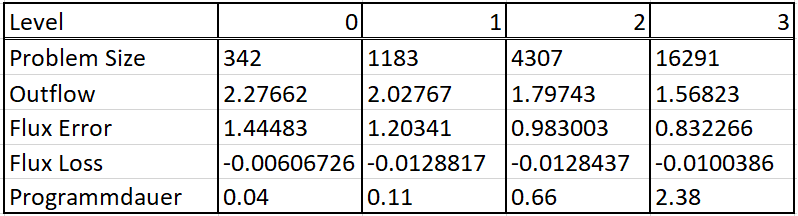
\includegraphics[width=0.99\textwidth]{../Aufgabe35/35_1_linear.png}}	 
\end{figure}

\begin{figure}[H]
	\centering
	\captionabove{Discretization = serendipity}
	\subfigure{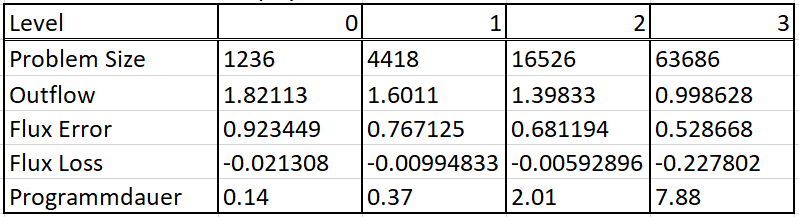
\includegraphics[width=0.99\textwidth]{../Aufgabe35/35_1_serendipity.png}}	 
\end{figure}
Man sieht sehr leicht, dass bei ähnlicher Problemgröße die quadratischen Ansatzelemente den linearen Ansatzelementen überlegen sind. Beispielsweise liefert der lineare Ansatz auf Level 1 (Problemgröße $\approx$ $1200$) einen Flux Error von $\approx 1.2$, während der quadratische Ansatz aus Level 0 (ebenfalls Problemgröße $\approx$ $1200$) mit einem Flux Error von $\approx 0.92$ genauer ausfällt. Diese Erkenntnis zieht sich auch bei anderen Wertepaaren durch die Tabelle.
Wir können dies auch von theoretischer Seite aus erklären:

Sei $V$ der Ansatzraum und $a(\cdot,\cdot)$ die zugehörige Bilinearform unseres aktuell gewählten Verfahrens (Finite Elemente bzw. Discontinuous Galerkin).
Wir erhalten dann im folgenden Lemma eine Aussage über die Güte unserer Approximationslösung:

\begin{Lemma}[Cea's Lemma]
  Sei $a(\cdot,\cdot)$ beschränkt und elliptisch, d.h.
  \begin{align*}
    |a(u,v)| \le C \|u'\| \|v'\|, \quad a(u,v) \ge c \| v'\|^2
    \quad \forall u,v \in V.
  \end{align*}
  Dann gilt für den Galerkin-Fehler $e_h = u-u_h$
  \begin{align*}
    \| e_h' \| \le \frac{C}{c} \inf\limits_{v_h \in V}
    \| u'-v_h' \|.
  \end{align*}
\end{Lemma}
Mit anderen Worten heißt das: Die berechnete Galerkin Approximation ist bezüglich einer geeigneten Norm eine Bestapproximation in unserem Ansatzraum $V$.
Die Vorraussetzungen des obigen Lemmas sind sowohl für die FEM als auch für das DGV erfüllt (vgl. Bericht 1-3 und
Eigenschaften von $ \asip(\cdot,\cdot) $ im ersten Kapitel).
Wir erhalten deshalb für quadratische Ansatzelemente auch eine etwas bessere Lösung, denn der Ansatzraum $V_h^{lin}$ der linearen Ansatzelemente ist natürlich Teilmenge des Ansatzraumes $V_h^{quad}$ der quadratischen Ansatzelemente. Da es sich bei der Finite Elemente Lösung um eine Galerkin-Approximation handelt und diese nach obigem Lemma eine Bestapproximation im zugehörigen Ansatzraum darstellt, kann die Lösung im größeren Ansatzraum $V_h^{quad}$ nur besser ausfallen.

Erstaunlich ist dabei, dass die Programmdauer bei minimal größerer Problemgröße und zudem besserer Genauigkeit bei den quadratischen Ansatzelementen für ungefähr gleiche Problemgröße dennoch meist geringer ausfällt als bei linearen Ansatzelementen. Zum Beispiel liefert Level 2 bei den lineare Ansatzelementen eine Programmdauer von 0.66 Sekunden, bei den quadratischen Ansatzelementen auf Level 1 aber nur von 0.37 Sekunden (Problemgröße $\approx 4350$ bei beiden).



\subsubsection{Aufgabe 35.2}
Als nächstes wollen wir uns dem DG-Ansatz widmen. Wir vergleichen hierbei  \unklar{EINLEITUNG???}

\begin{figure}[H]
	\centering
	\captionabove{symmetric}
	\subfigure{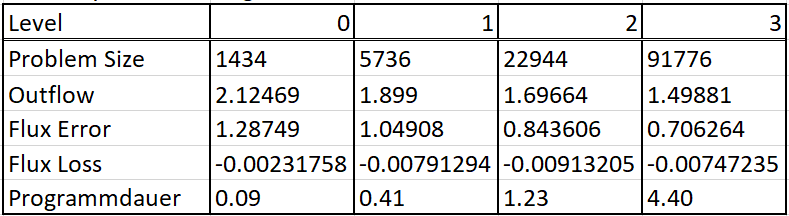
\includegraphics[width=0.99\textwidth]{../Aufgabe35/35_2_sym.png}}	 
\end{figure}


\begin{figure}[H]
	\centering
	\captionabove{non-symmetric}
	\subfigure{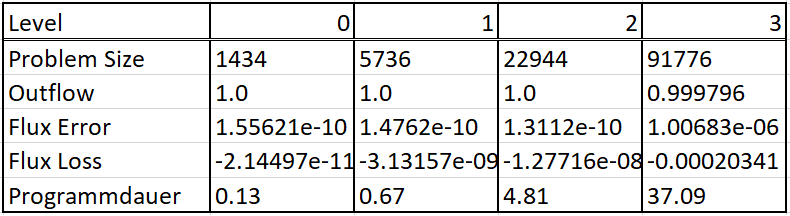
\includegraphics[width=0.99\textwidth]{../Aufgabe35/35_2_nonsym.png}}	 
\end{figure}

Wir wollen nun auf die Vor- und Nachteile bei symmetrischer und nicht-symmetrischer Konfiguration eingehen.
Schnell fällt ins Auge, dass die Ergebnisse des nicht-symmetrischen Verfahrens deutlich besser sind als mit symmetrischer Konfiguration. Während nämlich der Flux Error auf allen Leveln bei der symmetrischen Konfiguration nahe 1 ist, bewegen wir uns bei nicht-symmetrischer Konfiguration im Bereich von (sogar meist besser als) $10^{-6}$. Allerdings sieht man auch sehr schnell ein, dass dies nur auf Kosten der Programmdauer möglich ist. Während auf Level 3 der symmetrische Fall nur 4,4 Sekunden dauert, benötigt das nicht-symmetrische Verfahren sogar fast das 10-fache (ca. 40 Sekunden). 

\subsubsection{Aufgabe 35.3}
\begin{figure}[H]
	\centering
	\captionabove{deg = 2}
	\subfigure{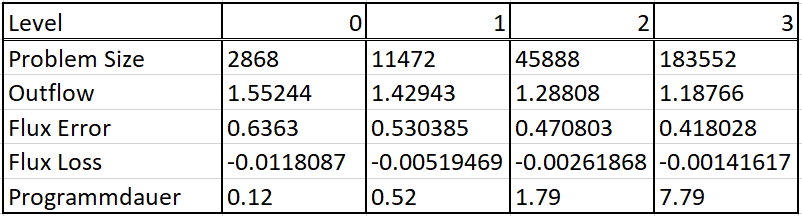
\includegraphics[width=0.99\textwidth]{../Aufgabe35/35_3_level.png}}	 
\end{figure}

Wie bei vorherigen Berichten berechnen wir auch hierzu mithilfe des Flux Errors eine Annäherung an die Konvergenzrate $p$ für den DG Ansatz mit quadratischen Ansatzelementen und symmetrischer Konfiguration.
Wir erhalten 
\begin{align*}
 \frac{e_l^{flux}}{e_{l+1}^{flux}} \approx 1.1508.
\end{align*}
Daraus erhalten wir die Konvergenzrate
\begin{align*}
  p \approx 0.2027.
\end{align*}

\subsubsection*{Penalty}
Wir betrachten nun den Einfluss des Parameters penalty auf das symmetrische DGV mit quadratischen Ansatzelementen.

\begin{figure}[H]
	\centering
	\captionabove{deg = 2, symmetrisch, level = 3}
	\subfigure{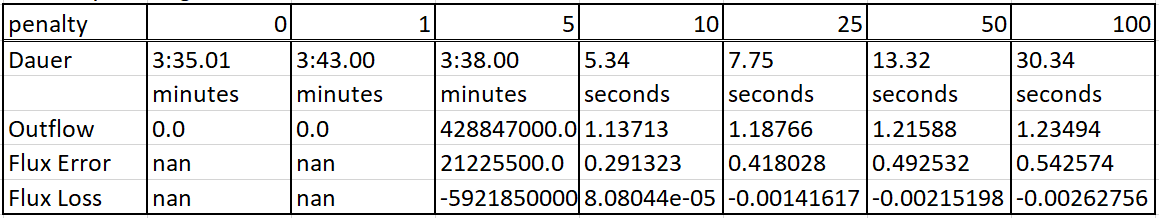
\includegraphics[width=0.99\textwidth]{../Aufgabe35/35_3_dauer.png}}	 
\end{figure}

Wie wir anhand der Tabelle sehen, ist das Verfahren für zu kleinen penalty instabil. Für penalty = 0,1,5 liefert das Verfahren keine brauchbaren Ergebnisse und benötigt eine lange Programmlaufzeit.
Für penalty = 10 erhalten wir eine gute Lösung bei relativ geringer Programmlaufzeit. Erhöhen wir nun den penalty noch weiter, so wird die Programmlaufzeit größer und zugleich die Lösung sogar schlechter. Es gilt also den penalty optimal in der Hinsicht zu wählen, dass das Verfahren stabil ist und der penalty trotzdem möglichst gering.



\subsubsection*{Problemgröße}
Wir wollen uns im Folgenden überlegen, wie die Anzahl der Unbekannten bei den unterschiedlichen Konfigurationen zustande kommen. 
Betrachten wir hierbei zunächst die FEM mit linearen Ansatzelementen stellen wir fest, dass sich die Problemgröße ungefähr in der Größenordnung der Anzahl der Knoten bewegt.
Wir können dies dadurch erklären, dass wir in unserem Ansatzraum für jeden Einzelknoten eine 'Hütchenfunktion' wählen können, welche einen Freiheitsgrad in der Gesamtapproximation ergibt.
Was wir allerdings noch beachten müssen, ist, dass die Dirichletränder bereits fest in unserem Ansatzraum $V_h(0)$ eingebaut sind, weswegen wir Knoten an Dirichleträndern nicht betrachten dürfen.
Es war uns leider nicht möglich die genaue Zusammensetzung der Problemgröße nachzuvollziehen. Was uns verwundert, ist, dass selbst auf verschiedenen Meshes mit gleich vielen Knoten bei gleichem Problem unterschiedliche Problemgrößen zustandekommen:
\begin{itemize}
  \item UnitSquare Lv4 = 289 (=Anzahl der Knoten)
  \item 2Triangles Lv4 = 321
  \item 8Triangles Lv3 = 353
  \item Square500  Lv0 = 342
\end{itemize} 
Sehr schön sieht man allerdings, dass wir pro Level ungefähr eine Vervierfachung der Problemgröße erhalten. Dies ist der Tatsache geschuldet, dass wir durch die Halbierung der Gitterweite viermal so viele Knoten erhalten.

Betrachten wir nun quadratische Ansatzelemente, erhalten wir auf Level 0 im Vergleich zu lineare Ansatzelementen ebenfalls etwa das Vierfache. Auch dies versuchen wir wieder anschaulich zu erklären: 
Wir können uns bei der Überlegung, wieviele Freiheitsgrade hinzukommen, einer einfachen Analogie bedienen: 
Durch die Wahl von quadratischen Ansatzelementen erhalten wir auf jeder Kante, also zwischen zwei Knoten, einen zusätzlichen Freiheitsgrad. Man kann also einsehen \textcolor{green}{??? BILD}, dass wir insgesamt in etwa so viele Freiheitsgrade erhalten, wie bei einem Gitter halber Gitterweite vorliegen. Das heißt wir erhalten beim Schritt von linearen zu quadratischen Ansatzelementen auch wieder ungefähr eine Vervierfachung des Ausgangswertes. Innerhalb der Diskretisierung mit quadratischen Ansatzelementen sehen wir erneut das Verhalten wie zuvor bei den linearen Ansatzelementen, d.h. eine Erhöhung des Levels um 1 hat eine Vervierfachung der Problemgröße zu folge.

\begin{figure}[H]
	\centering
	\captionabove{Problemgröße}
	\subfigure{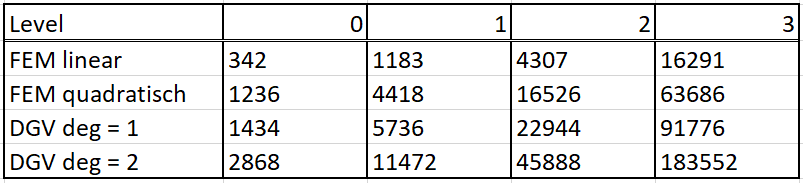
\includegraphics[width=0.99\textwidth]{../Aufgabe35/blub.png}}	 
\end{figure}

Betrachten wir nun das Discontinous Galerkin Verfahren. Wir müssen hierbei beachten, dass wir nun auch unstetige Ansätze erlauben. Es sind also auf den Knoten auch Sprungstellen erlaubt. Wir können uns auch hier einer einfachen Analogie bedienen und betrachten für jeden Knoten für jede anliegende Zelle einen eigenen Hilfsknoten. In unserem Fall erhalten wir bei linearen Ansatzelementen für jede Zelle gerade drei dieser Hilfsknoten (Square500 ist aus Dreiecken aufgebaut). Wir erhalten also für Level 0 (478 Zellen) gerade $3 \cdot 478 = 1434$ Freiheitsgrade. Mit steigendem Level erhalten dann exakt viermal so viele Freiheitsgrade, da bei Halbierung der Gitterweite sich die Zellenanzahl vervierfacht. 

Betrachten wir nun erneut den Schritt von deg = 1 auf deg = 2 können wir die gleiche Analogie wie bereits bei der FEM nutzen. Wir erhalten also bei den quadratischen Ansatzelementen jeweils auf den Kanten einen weiteren Freiheitsgrad. Nun ist aber auch dieser Parameter wieder unstetig wählbar. Mit dem gleichen Trick wie zuvor bei deg = 1 können wir uns also überlegen, dass wir nun auch für jede Kante für jede angrenzende Zelle einen Freiheitsgrad erhalten und so gerade auf das sechsfache der Zellenanzahl kommen (jede Zelle hat 3 Ecken und 3 Kanten).
Auch diese Werte lassen sich genau so in der Tabelle wiederfinden und wir können insgesamt die Verdopplung der Freiheitsgrade beim Schritt von deg = 1 auf deg = 2 feststellen.






% !TeX root = Bericht_main.tex
\subsection{Aufgabe 30}
In Aufgabe 30 betrachten wir nochmals die Konvektions-Diffusions-Reaktions-Gleichung 
\begin{align*}
	\partial_t c = \dive ( \kappa_c \nabla c - cq) + r(c)
\end{align*}
Im Vergleich zur letzten Aufgabe wollen wir nun aber den Reaktionsterm $r(c)$ ändern und so statt exponentiellem Wachstum, logistisches Wachstum betrachten. Während wir also zuvor noch $r(c) = Rc$ für ein $R \in \R$ gesetzt hatten, setzen wir nun $r(c) = r_0 c - r_1 c^2$ für $r_0,r_1 > 0$
\newline
Dazu sind wir wie folgt vorgegangen:
SCREENSHOT

% !TeX root = Bericht_main.tex

\subsection{Aufgabe 31}

In Aufgabe 31 versuchen wir Schritt für Schritt eine sinnvolle Wahl für die Feinheit von Orts- bzw. Zeitdiskretisierung herauszufinden. Dazu ermitteln wir abhängig vom Verfeinerungslevel $level = 0,1,2$ eine sinnvolle Zeitschrittweite, sodass der Fehler der Zeitdiskretisierung kleiner als der Ortsfehler ist und der Startwert des Newton-Verfahrens so gut ist, dass die Newton-Konvergenz quadratisch ist. 
Wir vergleichen dazu die Masse der Konzentration in einem Plot für das exponentielle Wachstum mit $ Reaction = 2.5 $

\begin{figure}[H]
	\centering
	\captionabove{Vergleich der Masse für unterschiedliche Zeitdiskretisierungen}
	\subfigure[auf Level = 0]{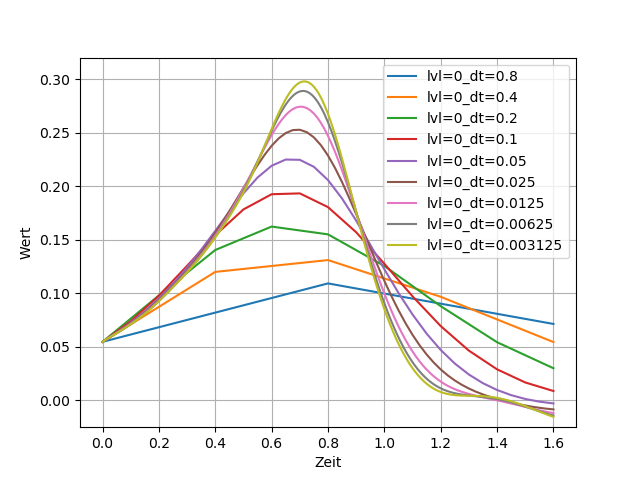
\includegraphics[width=0.85\textwidth]{../Aufgabe31/Maxdiff/zeitvergleich_lvl=0_plot.png}}
\end{figure}
\begin{figure}[H]
	\centering
	\subfigure[auf Level = 1]{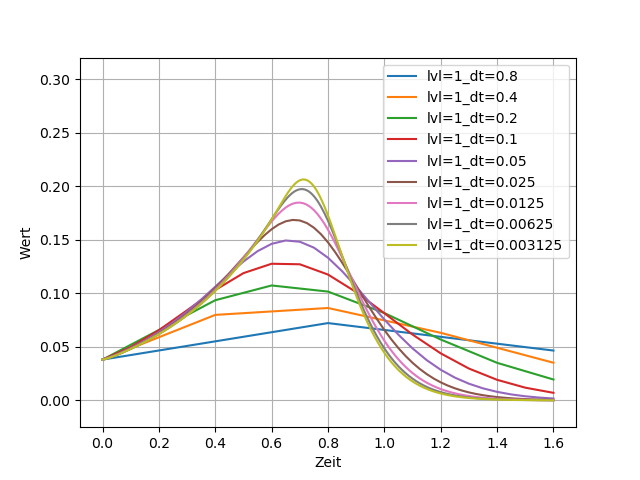
\includegraphics[width=0.85\textwidth]{../Aufgabe31/Maxdiff/zeitvergleich_lvl=1_plot.png}}
\end{figure}
\begin{figure}[H]
	\centering
	\subfigure[auf Level = 2]{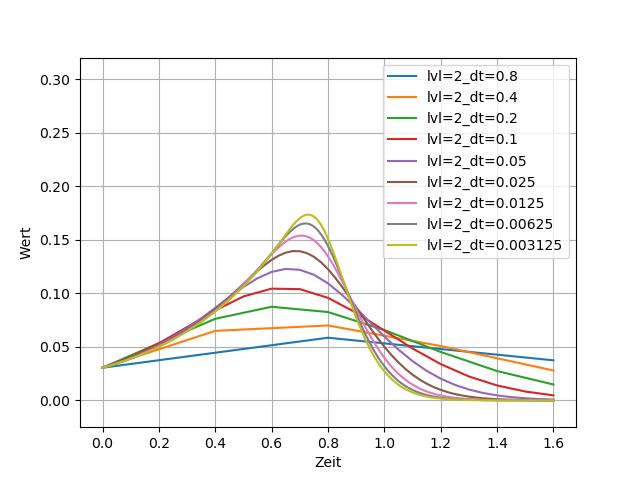
\includegraphics[width=0.85\textwidth]{../Aufgabe31/Maxdiff/zeitvergleich_lvl=2_plot.png}}
\end{figure}

Um zusätzlich zum Fehler der Zeitdiskretisierung auch den Fehler der Ortsdiskretisierung abschätzen zu können, ist es zudem hilfreich auch die verschiedenen Masseplots für eine fest gewählte Zeitdiskretisierung auf den unterschiedlichen Levels zu vergleichen:
 
 \begin{figure}[H]
 	\centering
 	\captionabove{Vergleich der Masse für $Level = 1,2,3$}
 	\subfigure[mit $dt = 0.8$]{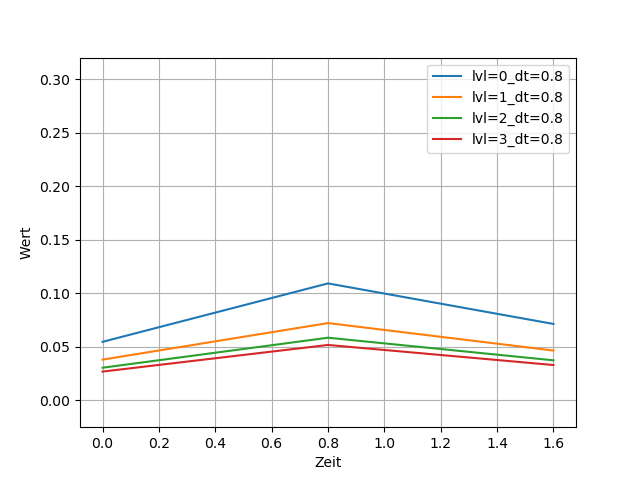
\includegraphics[width=0.32\textwidth]{../Aufgabe31/Maxdiff/3vergleich_dt=08_plot.png}}
 	\subfigure[mit $dt = 0.4$]{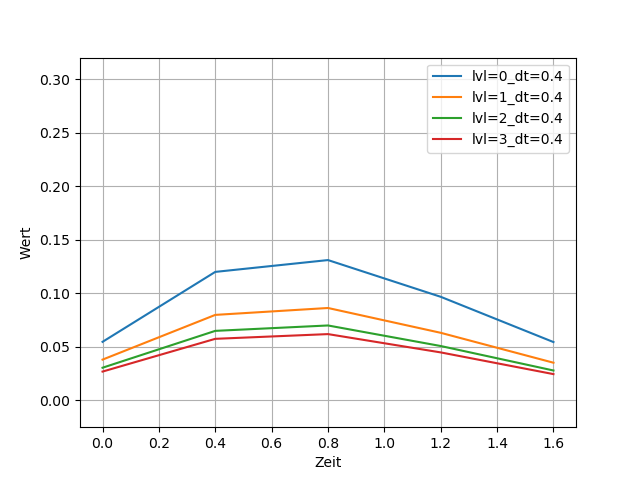
\includegraphics[width=0.32\textwidth]{../Aufgabe31/Maxdiff/3vergleich_dt=04_plot.png}}
 	\subfigure[mit $dt = 0.2$]{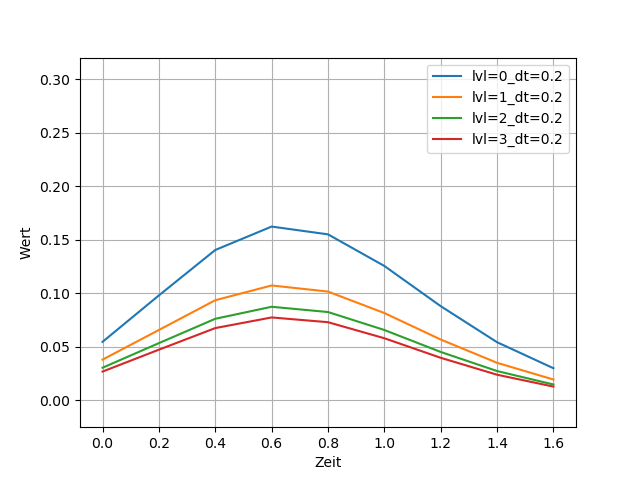
\includegraphics[width=0.32\textwidth]{../Aufgabe31/Maxdiff/3vergleich_dt=02_plot.png}}
 	\subfigure[mit $dt = 0.1$]{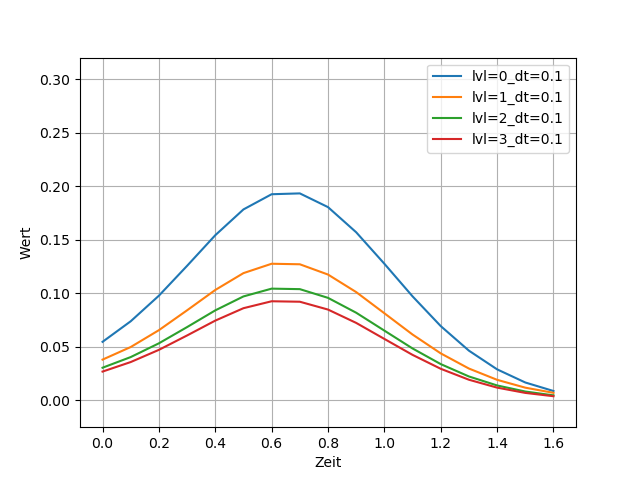
\includegraphics[width=0.32\textwidth]{../Aufgabe31/Maxdiff/3vergleich_dt=01_plot.png}}
 	\subfigure[mit $dt = 0.05$]{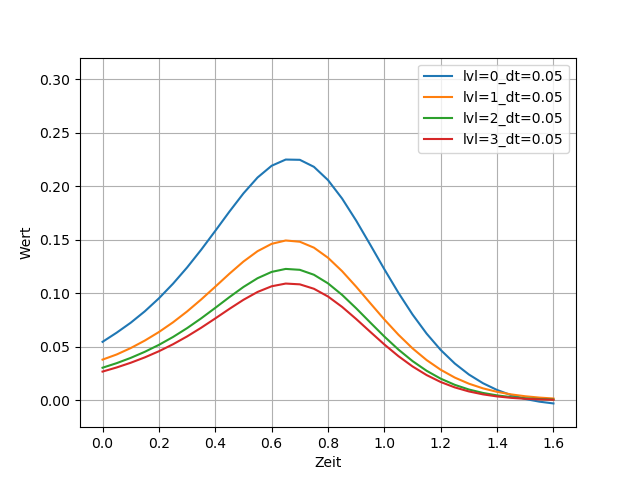
\includegraphics[width=0.32\textwidth]{../Aufgabe31/Maxdiff/3vergleich_dt=005_plot.png}}
 	\subfigure[mit $dt = 0.025$]{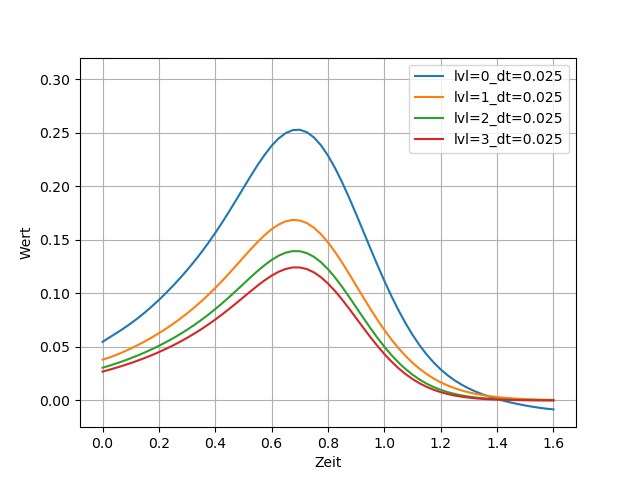
\includegraphics[width=0.32\textwidth]{../Aufgabe31/Maxdiff/3vergleich_dt=0025_plot.png}}
 	\subfigure[mit $dt = 0.0125$]{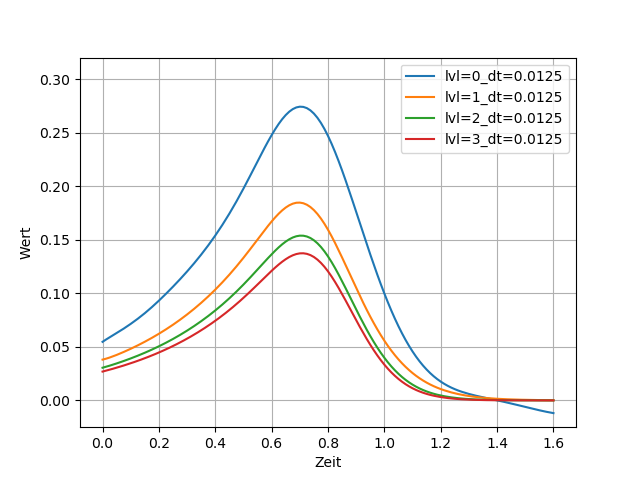
\includegraphics[width=0.32\textwidth]{../Aufgabe31/Maxdiff/3vergleich_dt=00125_plot.png}}
 	\subfigure[mit $dt = 0.00625$]{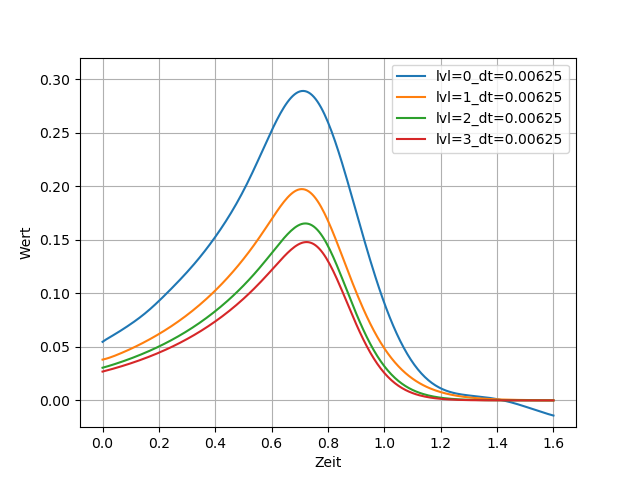
\includegraphics[width=0.32\textwidth]{../Aufgabe31/Maxdiff/3vergleich_dt=000625_plot.png}}
 \end{figure}

Ziel ist es nun, die Fehler der Zeit- bzw. Orstdiskretisierung für für ein bestimmtes Level mit einer bestimmten Schrittweite zu schätzen. 
Dazu vergleichen wir für den Ortsfehler die Masse der aktuellen Zeitschrittweite und des aktuellen Levels mit der Masse der aktuellen Zeitschrittweite und des nächstfeineren Levels.
Für den Fehler der Zeitdiskretisierung vergleichen wir die Masse der aktuellen Zeitschrittweite und des aktuellen Levels mit der Masse des aktuellen Levels und der nächstfeineren Zeitschrittweite.
Als erste Annäherung an eine Metrik betrachten wir jeweils den maximalen Unterschied der einzelnen Massewerte zu den verschiedenen Zeitschritten $t$.
Bei dem Fehler der Ortsdiskretisierung lassen wir, wie oben beschrieben, die Zeitschrittweite fest und erhalten so für genau dieselben Zeitschritte $t$ entsprechende Massewerte. Somit erhalten wir 
\begin{align*}
	r_{Ort}  \approx \max_{t \in \{t_0 = 0,t_1,...,t_n=1.6 \}  } |m_{lvl}(t) - m_{lvl + 1} (t) |
\end{align*}
Bei dem Fehler der Zeitdiskretisierung haben wir zwar bei der feineren Schrittweite theoretisch mehr Werte zu Verfügung, wir vergleichen aber auch hier nur an den Zeitschritten $t$ der gröberen Schrittweite, da wir sonst die Zwischenwerte interpolieren müssten:
\begin{align*}
r_{Zeit}  \approx \max_{t \in \{t_0 = 0,t_1,...,t_n=1.6 \}  } |m_{dt}(t) - m_{dt/2} (t) |
\end{align*}
Wir erhalten so folgende Werte als Heatmap:
\begin{figure}[H]
	\centering
	\captionabove{Annäherungen an Fehler der Zeit- und Ortsdiskretisierung}
	\subfigure[auf Level = 0]{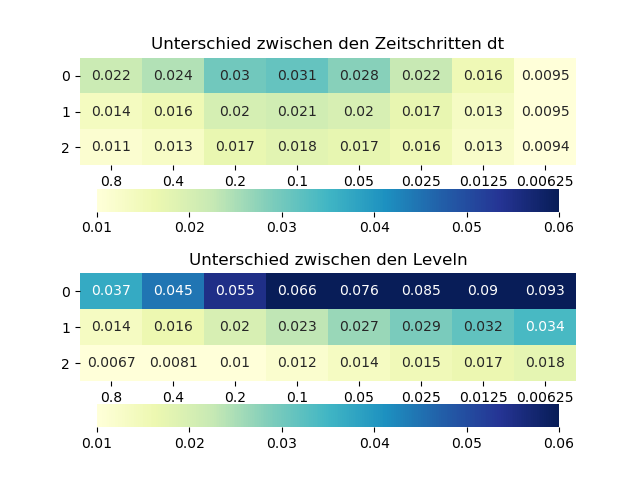
\includegraphics[width=0.85\textwidth]{../Aufgabe31/Maxdiff/Heatmapblub.png}}
\end{figure}
Dabei sind die Werte in 'Unterschied zwischen den Zeitschrittschritten' gerade der oben erklärte Wert $r_{Zeit}$ und die Werte in  'Unterschiede zwischen den Leveln' gerade der Wert $r_{Ort}$

Damit können wir folgende sinnvolle Werte für die Zeitschrittweite herauslesen:
\begin{figure}[H]
	\centering
	\captionabove{Sinnvolle Werte für die Zeitschrittweite abhängig vom Level}
	\subfigure[auf Level = 0]{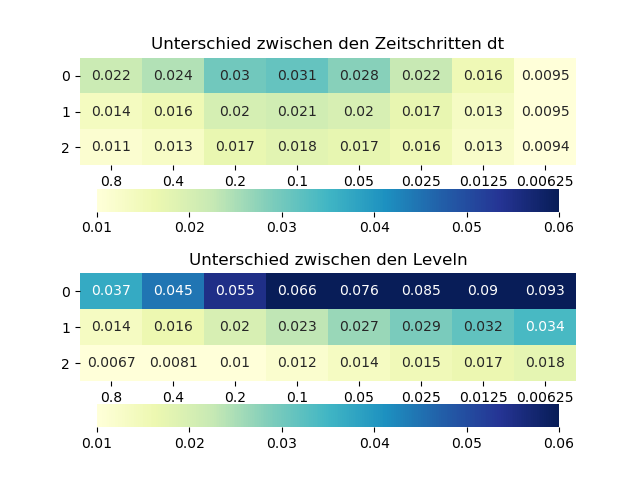
\includegraphics[width=0.85\textwidth]{../Aufgabe31/Maxdiff/Heatmapblub1.png}}
\end{figure}
Für Level 0  reicht uns bereits die geringste Zeitschrittweite $dt = 0.8$, anders ausgedrückt, der Fehler der Orstdiskretisierung ist schlichtweg zu groß. Für Level 1 erhalten wir $dt= 0.1$ als sinnvolle Wahl, denn für eine geringere Zeitschrittweite überwiegt der Fehler der Orstdiskretisierung, für eine größere Wahl von dt ist hingegen der Fehler der Zeitdiskretisierung nicht mehr kleiner als der Fehler der Fehler der Orstdiskretisierung.
Nach analogem Auswahlverfahren erhalten wir für Level 2 $dt = 0.0125$ als sinnvolle Wahl für die Zeitschrittweite.





% !TeX root = Bericht_main.tex
\newpage
\subsection{Aufgabe 32}
In Aufgabe 32 beschäftigen wir uns nochmal mit dem Grenzfall 
Diffusion $\to 0$. Zunächst sei dabei die Reaktionsrate $r=5$. Dabei werden wir nun das Streamline Diffusion Verfahren (SDV) verwenden (vgl. Theorieteil Abschnitt 1.4).

\begin{figure}[H]
	\centering
	\captionabove{Vergleich unterschiedlicher Verfahren bei Diffusion 0.00001 zum Zeitpunkt $t=1$}
	\subfigure[FEM lv2]{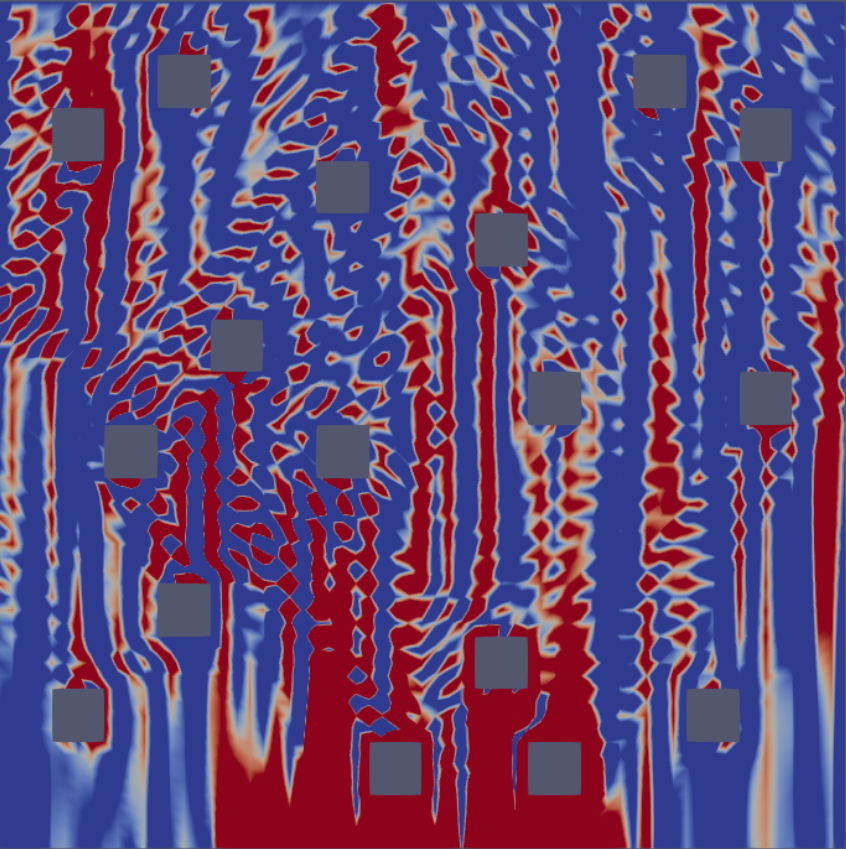
\includegraphics[width=0.32\textwidth]{../Aufgabe27/b/reaction=5_diffusion=1e-05/animation40.png}}	 
	\subfigure[Serendipity lv2]{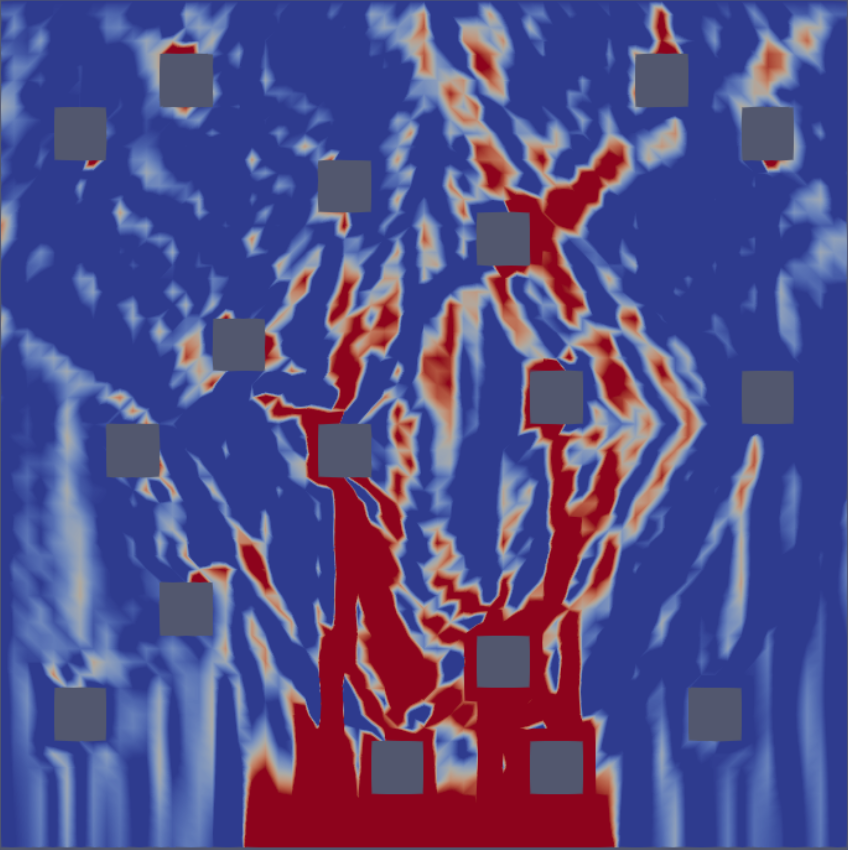
\includegraphics[width=0.32\textwidth]{../Aufgabe27/c/serendipity_lvl=2_reaction=5_diffusion=1e-05/animation40.png}}
    \subfigure[Serendipity lv3] {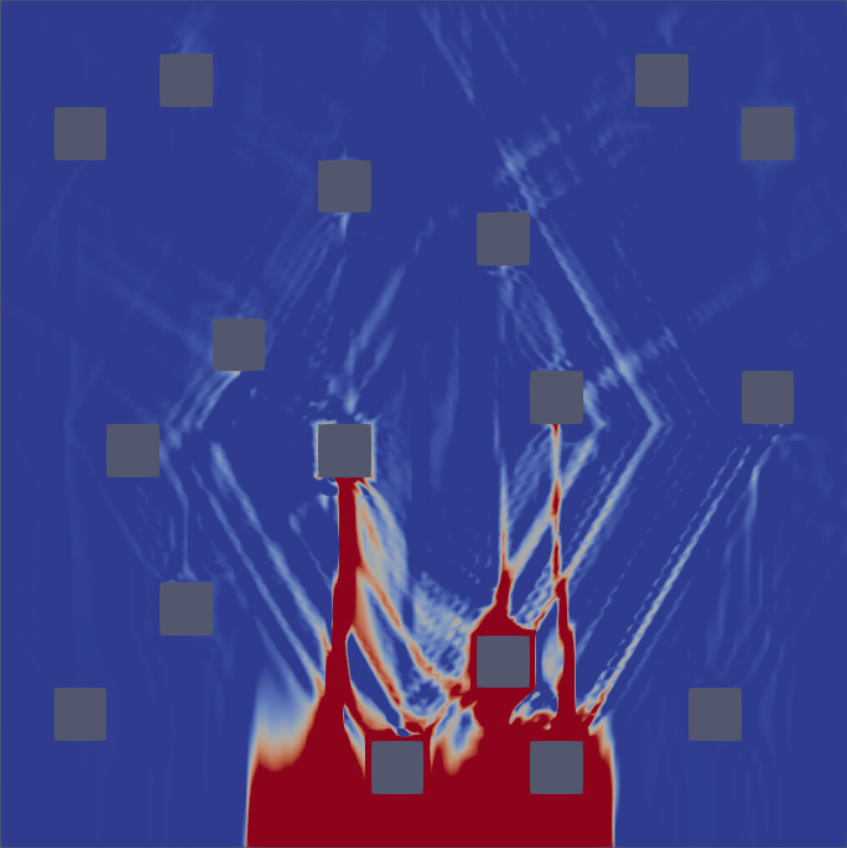
\includegraphics[width=0.32\textwidth]{../Aufgabe27/c/serendipity_lvl=3_reaction=5_diffusion=1e-05/animation40.png}}
    \subfigure[SDV Delta 0.025]{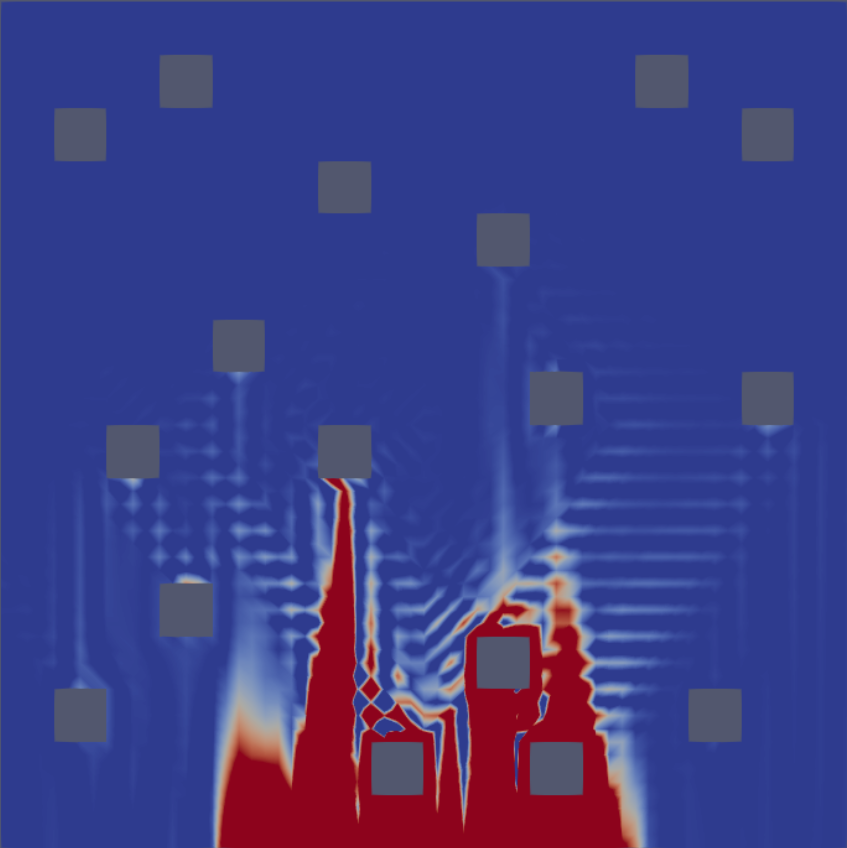
\includegraphics[width=0.32\textwidth]{../Aufgabe32/delta=0.025_diffusion=1e-05/animation40.png}}
    \subfigure[SDV Delta 0.1]{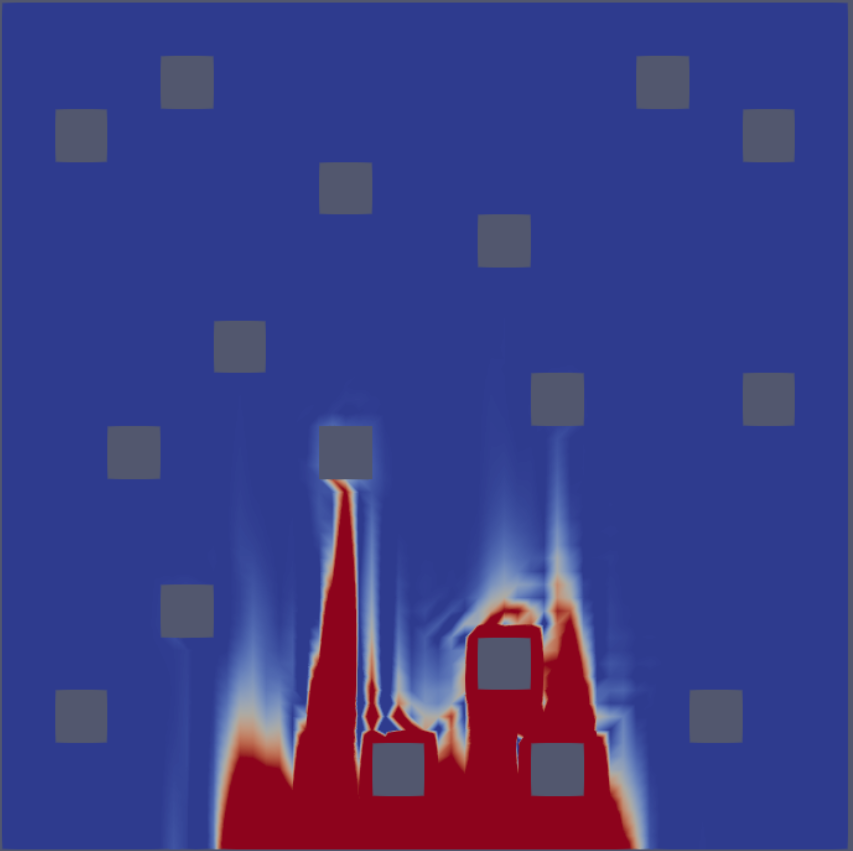
\includegraphics[width=0.32\textwidth]{../Aufgabe32/delta=0.1_diffusion=1e-05/animation40.png}}  
    \subfigure[SDV Delta 5]{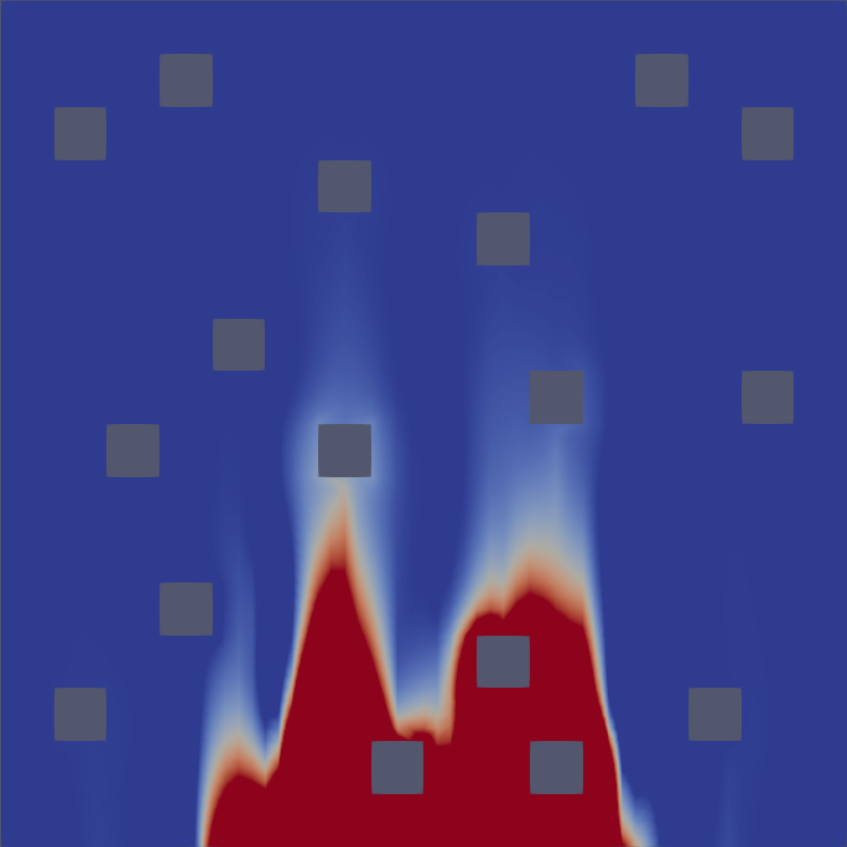
\includegraphics[width=0.32\textwidth]{../Aufgabe32/delta=5_diffusion=1e-05/animation40.png}}
\end{figure}

Wie wir anhand der Bilder zum Zeitpunkt $t=1$ erkennen können, eignen sich unsere bisherigen Verfahren (FEM und Serendipity) nicht für die sehr geringe Diffusion 0.00001. Im Gegensatz dazu steht das Streamline Diffusion Verfahren. Dabei erzeugen wir mithilfe von $\delta_K$ eine 'künstliche' Diffusion. Schon bei einem $\delta_K$ in der Größenordnung unserer Gitterweite ($\approx 0.025$)
erhalten wir eine deutlich bessere Lösung, als zuvor noch mit den bisherigen Verfahren. Bei einem sehr großen Delta 
($\approx 5$) sieht unsere Lösung glatt aus. Dies ist der Tatsache geschuldet, dass wir durch das große Delta auch eine große 'künstliche' Diffusion erzeugt haben. Noch deutlicher sieht man das bei noch geringeren Diffusionen:

\begin{figure}[H]
	\centering
	\captionabove{Vergleich unterschiedlicher Verfahren bei Diffusion 0.000001 zum Zeitpunkt $t=1$}
	\subfigure[FEM lv2]{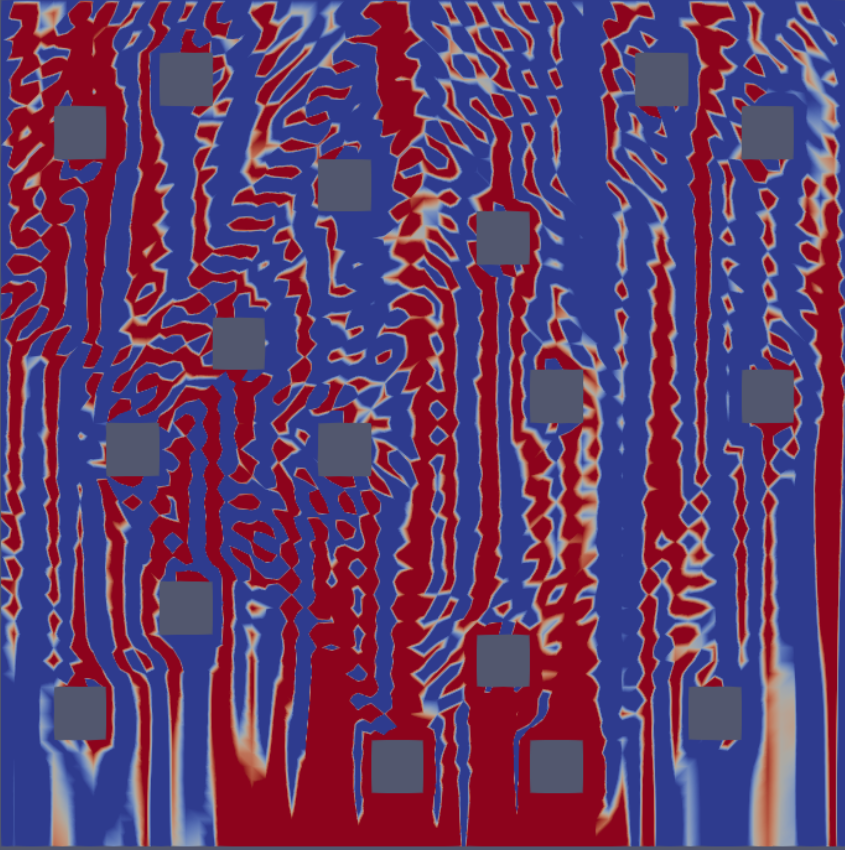
\includegraphics[width=0.32\textwidth]{../Aufgabe27/b/reaction=5_diffusion=1e-06/animation40.png}}	 
	\subfigure[Serendipity lv2]{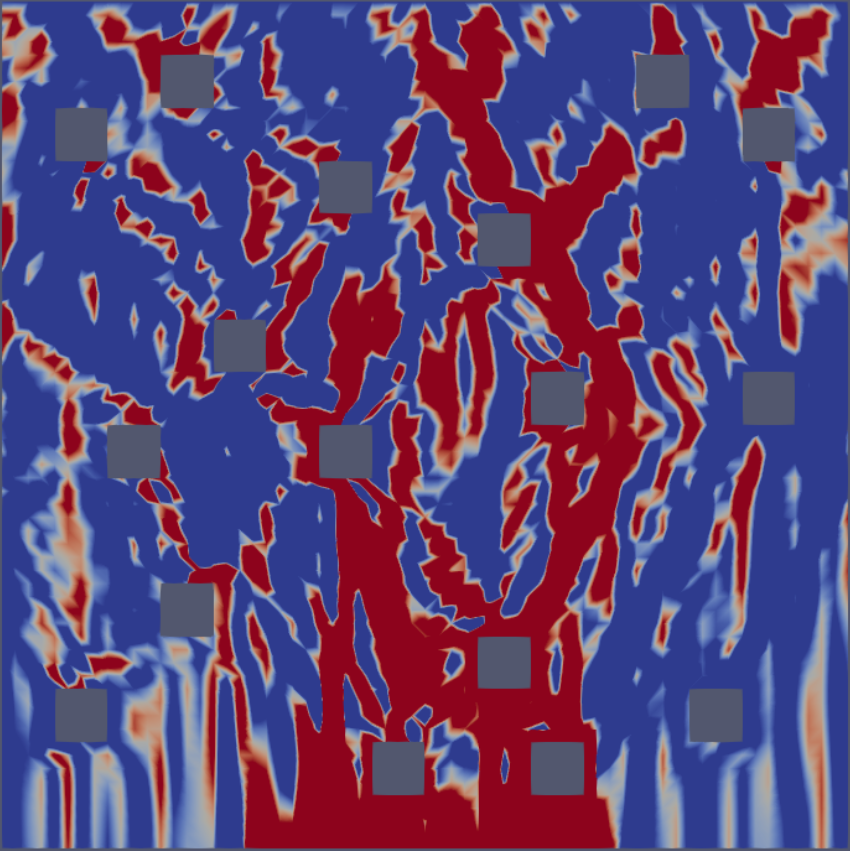
\includegraphics[width=0.32\textwidth]{../Aufgabe27/c/serendipity_lvl=2_reaction=5_diffusion=1e-06/animation40.png}}
	\subfigure[Serendipity lv3] {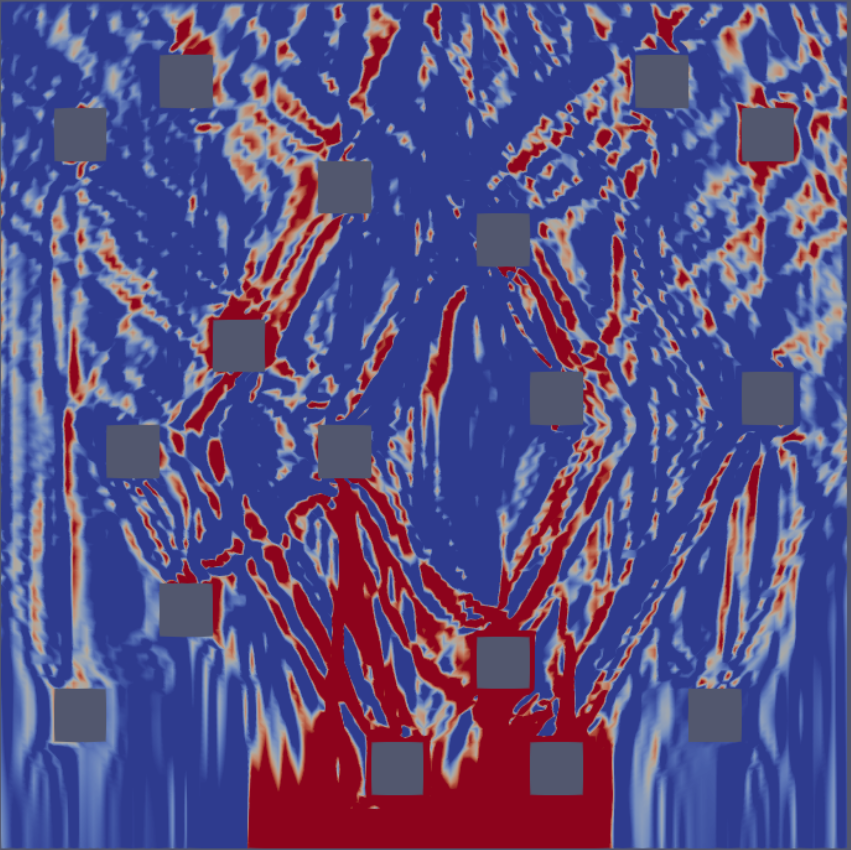
\includegraphics[width=0.32\textwidth]{../Aufgabe27/c/serendipity_lvl=3_reaction=5_diffusion=1e-06/animation40.png}}
	\subfigure[SDV Delta 0.025]{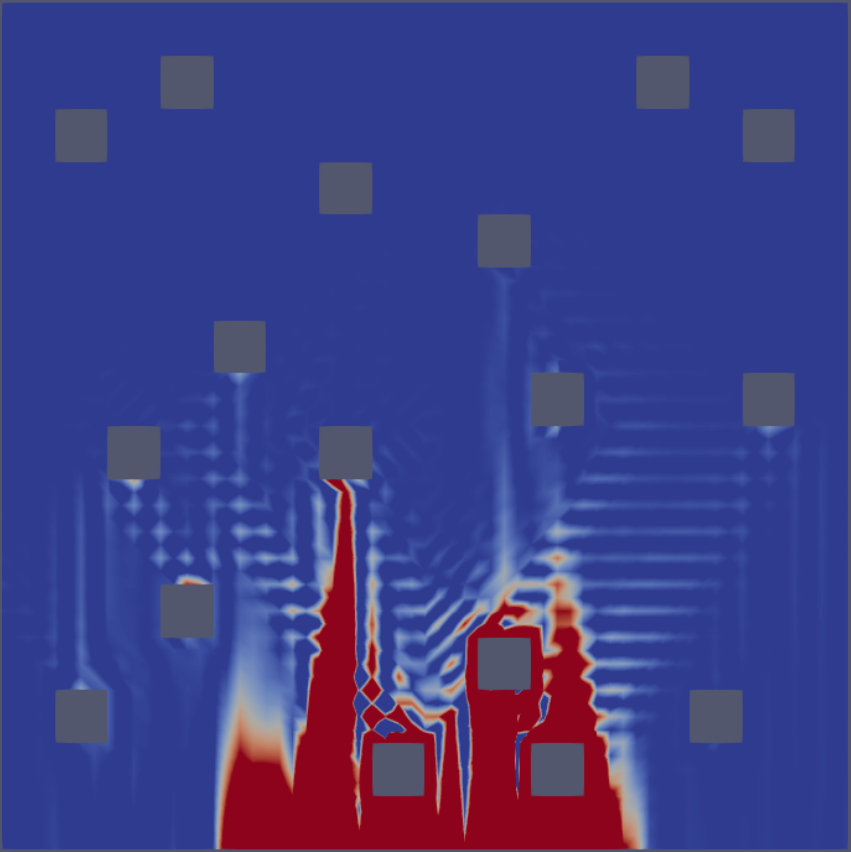
\includegraphics[width=0.32\textwidth]{../Aufgabe32/delta=0.025_diffusion=1e-06/animation40.png}}
	\subfigure[SDV Delta 0.1]{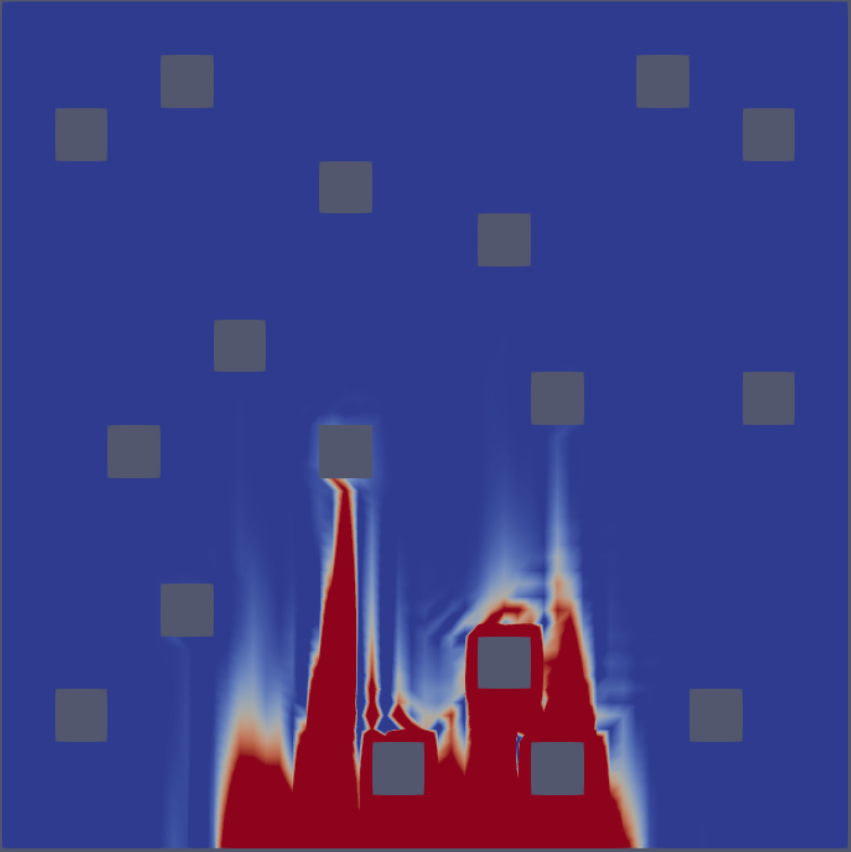
\includegraphics[width=0.32\textwidth]{../Aufgabe32/delta=0.1_diffusion=1e-06/animation40.png}}  
	\subfigure[SDV Delta 5]{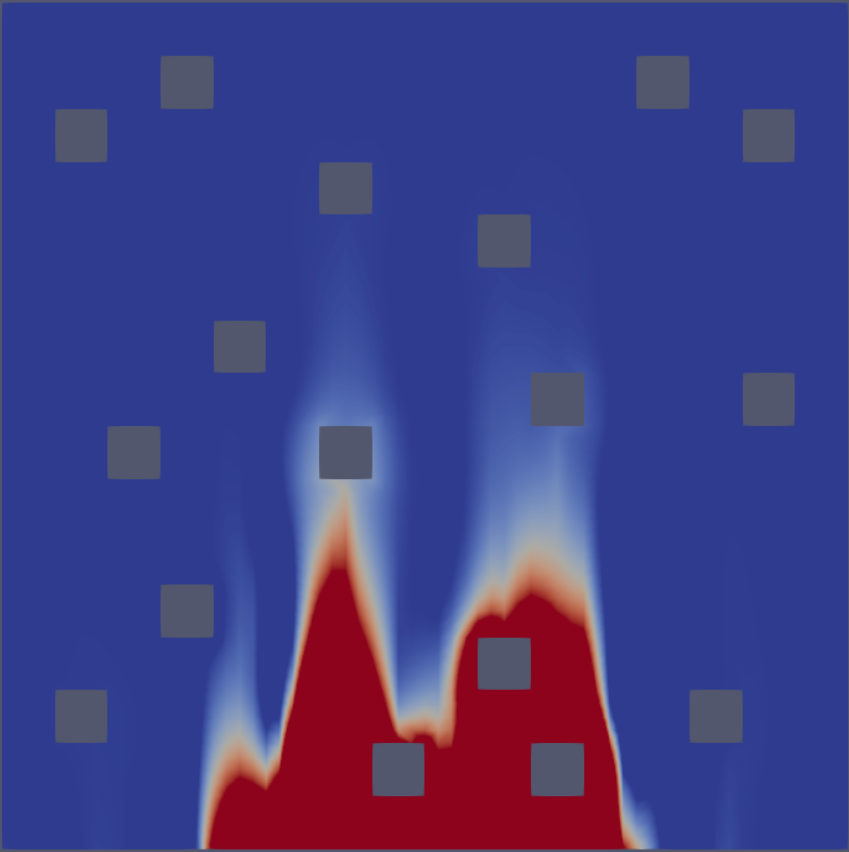
\includegraphics[width=0.32\textwidth]{../Aufgabe32/delta=5_diffusion=1e-06/animation40.png}}
\end{figure}

Insgesamt haben wir damit durch die unstetige Wahl der Testfunktionen im SDV ein bereits brauchbares Verfahren für das Problem Diffusion $\to 0$ gefunden, bei dem die bisherigen Verfahren  starke Oszillationen aufwiesen. 
Wir können nun noch für die Reaktionsrate $r=0$ unsere Lösungen der Konvektions-Diffusions-Reaktions-Gleichung für sehr kleine Diffusion mit der Lösung des reinen Transportproblems vergleichen.






\end{document}

